%%
%% This is file `tikzposter-template.tex',
%% generated with the docstrip utility.
%%
%% The original source files were:
%%
%% tikzposter.dtx  (with options: `tikzposter-template.tex')
%%
%% This is a generated file.
%%
%% Copyright (C) 2014 by Pascal Richter, Elena Botoeva, Richard Barnard, and Dirk Surmann
%%
%% This file may be distributed and/or modified under the
%% conditions of the LaTeX Project Public License, either
%% version 2.0 of this license or (at your option) any later
%% version. The latest version of this license is in:
%%
%% http://www.latex-project.org/lppl.txt
%%
%% and version 2.0 or later is part of all distributions of
%% LaTeX version 2013/12/01 or later.
%%


\documentclass{tikzposter} %Options for format can be included here

\usepackage{showframe}
\usepackage{todonotes}
\usepackage[ruled]{algorithm2e}
\usepackage[tikz]{bclogo}
\usepackage{lipsum}
\usepackage{amsmath}
\usepackage{algorithm}
\usepackage{algorithmic}
\usepackage{booktabs}
\usepackage{longtable}
\usepackage[absolute]{textpos}
\usepackage[it]{subfigure}
\usepackage{graphicx}
\usepackage{cmbright}
%\usepackage[default]{cantarell}
%\usepackage{avant}
%\usepackage[math]{iwona}
\usepackage[math]{kurier}
\usepackage[T1]{fontenc}


%% add your packages here
\usepackage{hyperref}
% for random text
\usepackage{lipsum}
\usepackage[english]{babel}
\usepackage[pangram]{blindtext}
\colorlet{backgroundcolor}{blue!10}

 % Title, Author, Institute
\title{Flip 00 project final report}
\author{Jin Chen}
\institute{ HuNan University, China
}
%\titlegraphic{logos/tulip-logo.eps}

%Choose Layout
\usetheme{Wave}

%\definebackgroundstyle{samplebackgroundstyle}{
%\draw[inner sep=0pt, line width=0pt, color=red, fill=backgroundcolor!30!black]
%(bottomleft) rectangle (topright);
%}
%
%\colorlet{backgroundcolor}{blue!10}

\begin{document}


\colorlet{blocktitlebgcolor}{blue!23}

 % Title block with title, author, logo, etc.
\maketitle

\begin{columns}
 % FIRST column
\column{0.5}% Width set relative to text width

%%%%%%%%%% -------------------------------------------------------------------- %%%%%%%%%%
 %\block{Main Objectives}{
%  	      	\begin{enumerate}
%  	      	\item Formalise research problem by extending \emph{outlying aspects mining}
%  	      	\item Proposed \emph{GOAM} algorithm is to solve research problem
%  	      	\item Utilise pruning strategies to reduce time complexity
%  	      	\end{enumerate}
%%  	      \end{minipage}
%}
%%%%%%%%%% -------------------------------------------------------------------- %%%%%%%%%%


%%%%%%%%%% -------------------------------------------------------------------- %%%%%%%%%%
\block{Introduction}{
    After a month of making scientific observations 
    and taking careful measurements, 
    can determined that 900 ghouls, ghosts, and goblins.
    The raw dataset contains train set with \emph{371} %modify as your true values
    samples and \emph{529} unlabeled samples as test set.
    Through the train data, find the relationship
    between the attributes and species, 
    and then identify the ghastly creatures.
    The following is the attributes list of data:
    \vspace{.5cm}
  	\begin{description}
  		\item[id] id of the creature
  		\item[bone\_length] average length of bone in the creature, 
  		normalized between \emph{0} and \emph{1}
  		\item[rotting\_flesh] percentage of rotting flesh in the creature
  		\item[hair\_length] average hair length, 
  		normalized between \emph{0} and \emph{1}
  		\item[has\_soul] percentage of soul in the creature
  		\item[Color] dominant color of the creature: 
  		\emph{white},\emph{black},\emph{clear},
  		\emph{blue},\emph{green},\emph{blood}
  		\item[type] target variable: 
  		\emph{Ghost}, \emph{Goblin}, and \emph{Ghoul}
  	\end{description}
    \vspace{.3cm}
}
%%%%%%%%%% -------------------------------------------------------------------- %%%%%%%%%%


%%%%%%%%%% -------------------------------------------------------------------- %%%%%%%%%%
\block{Data Visualization}{
	The following figures show
	the distribution of the data. 
	The pairplot shows that 
	data is distributed normally. 
	and most pairs are widely scattered  
	but some of them show clusters.
	Through correlogram can gain that
	it is no obvious linear relationship 
	between variables.
	And boxplot shows the outliers are very small,
	which can be ignored.
	\vspace{.5cm}
	\begin{center}
		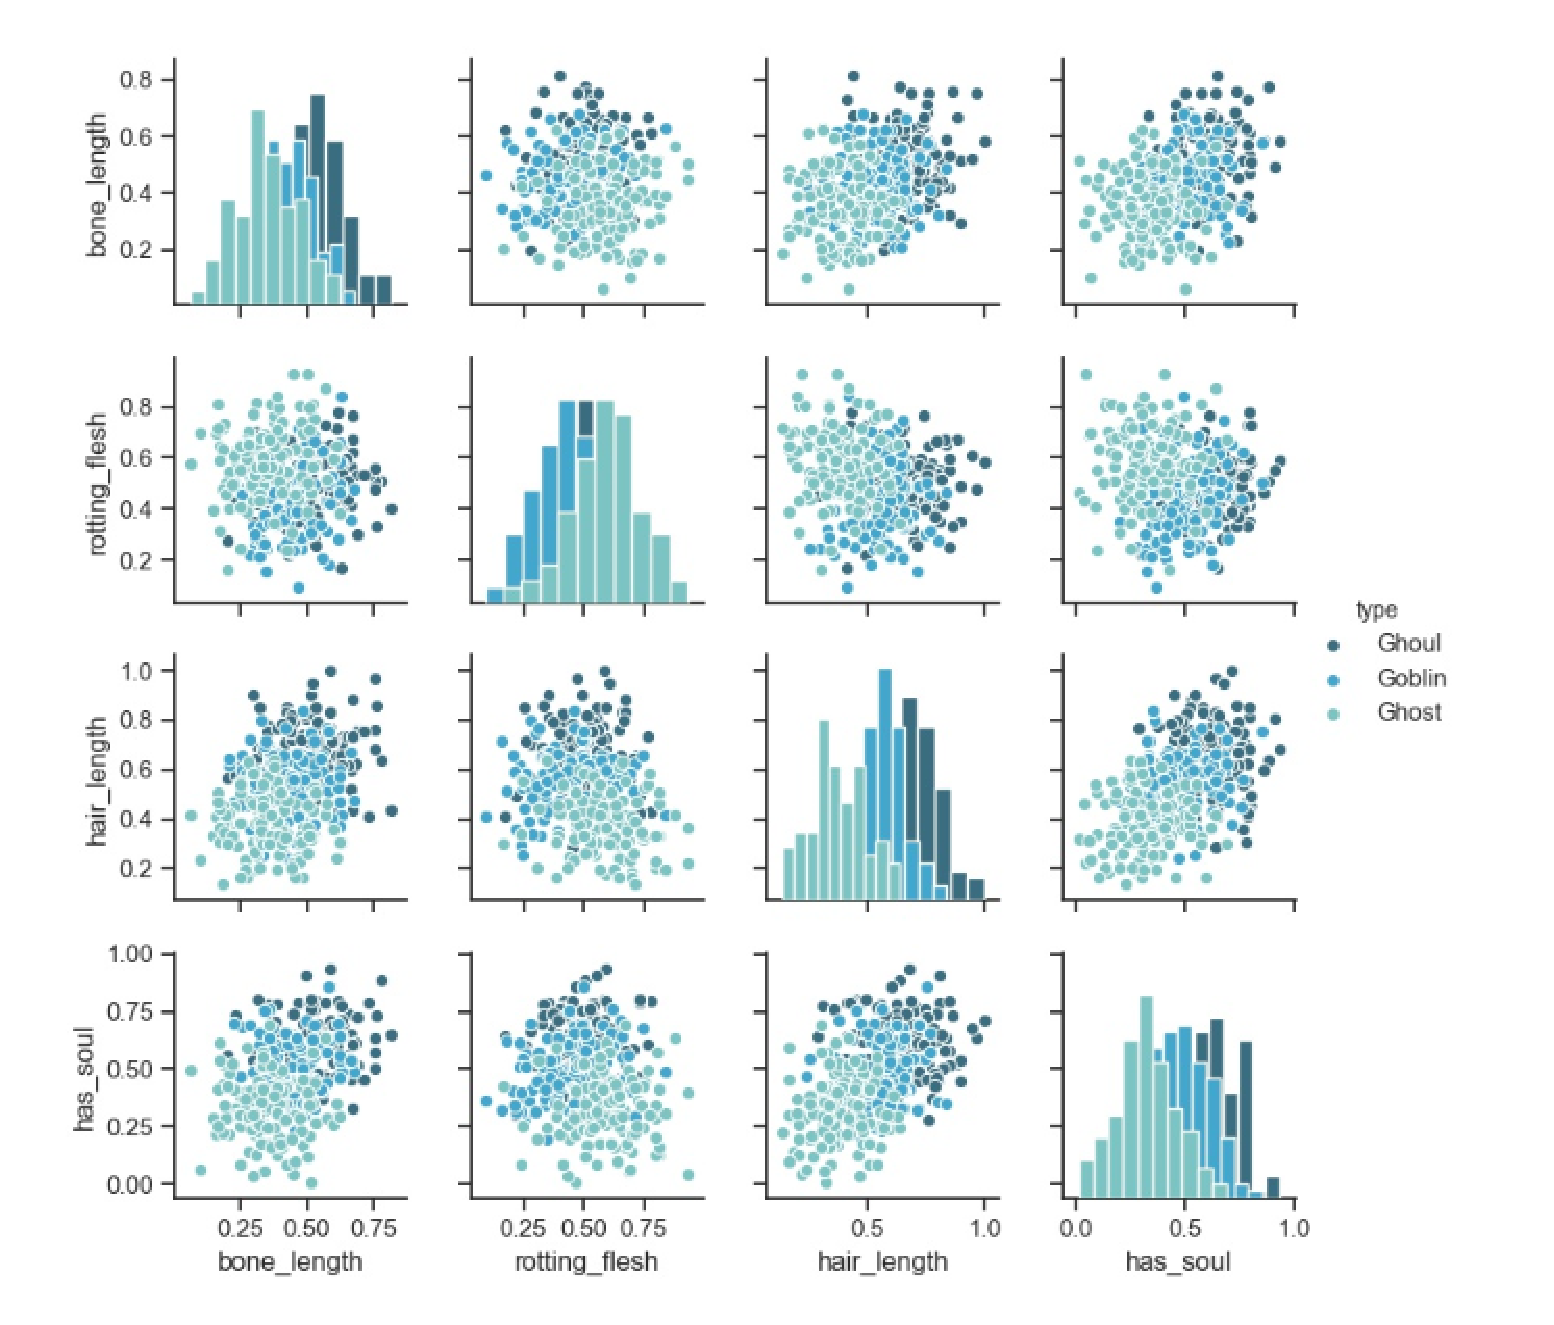
\includegraphics[width=.3\linewidth]{figures/pairplot.eps}
		\quad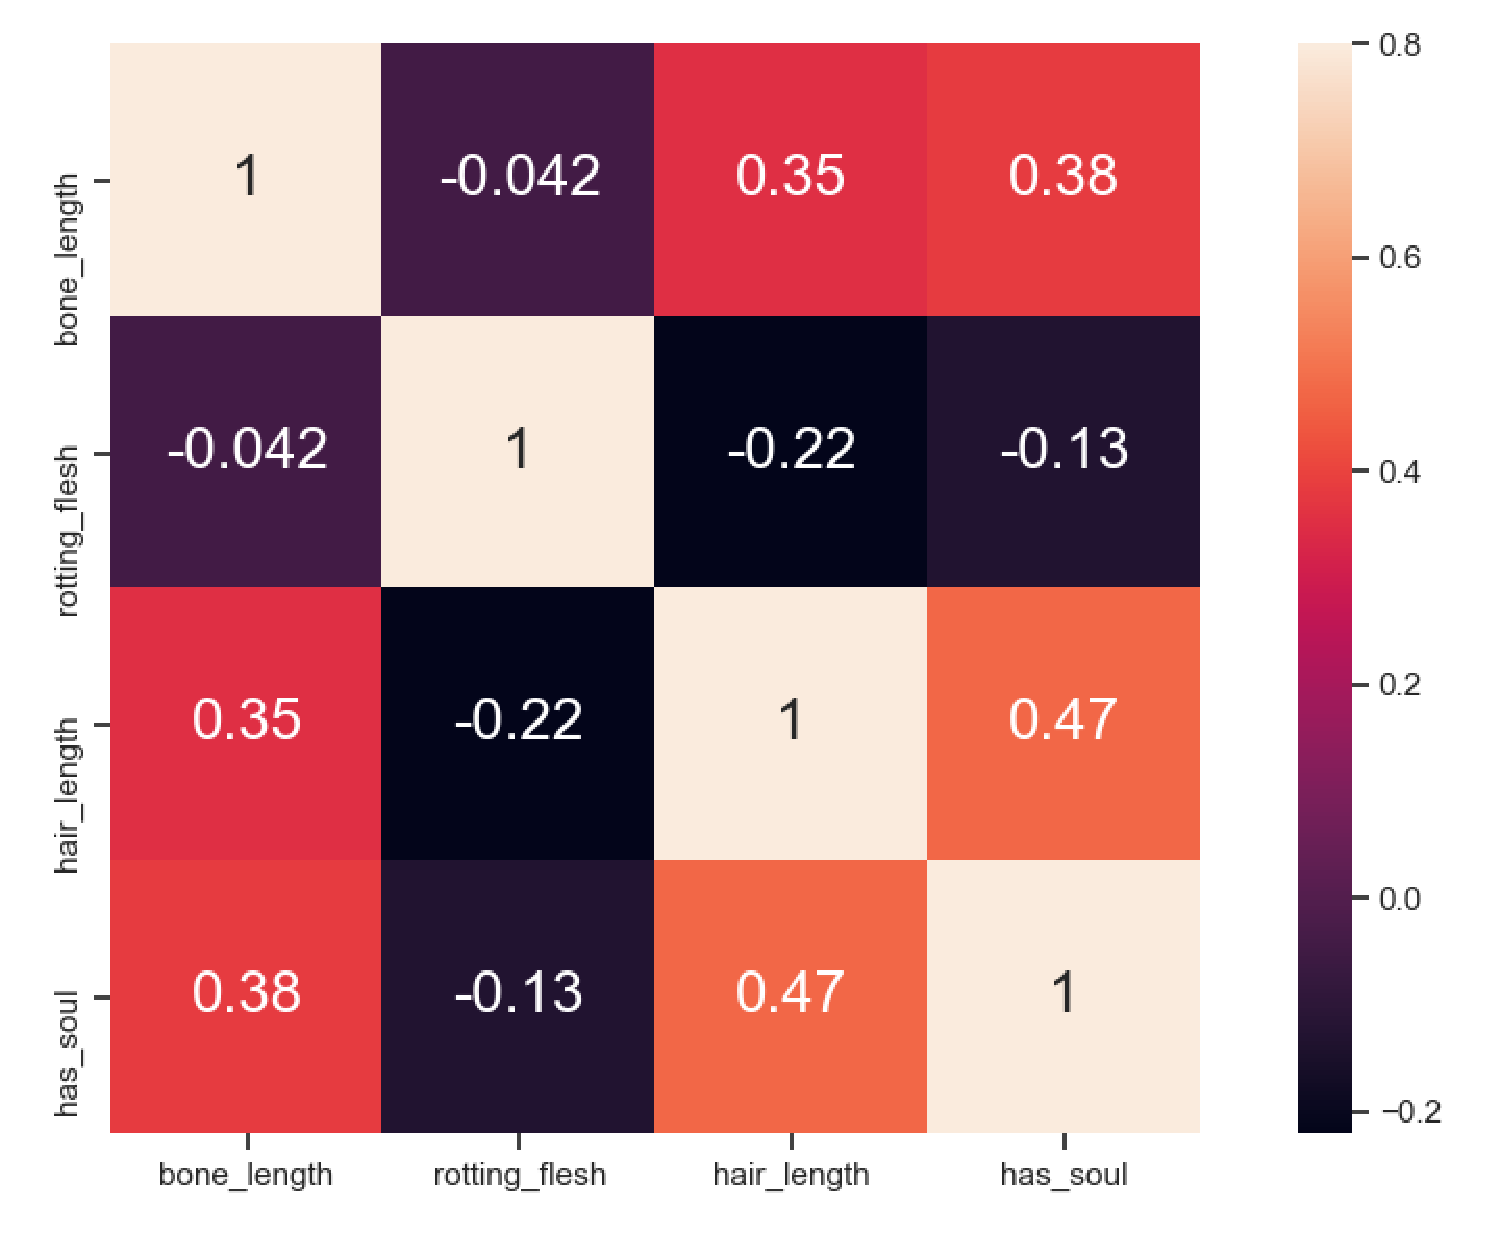
\includegraphics[width=.3\linewidth]{figures/corr.eps}
		\quad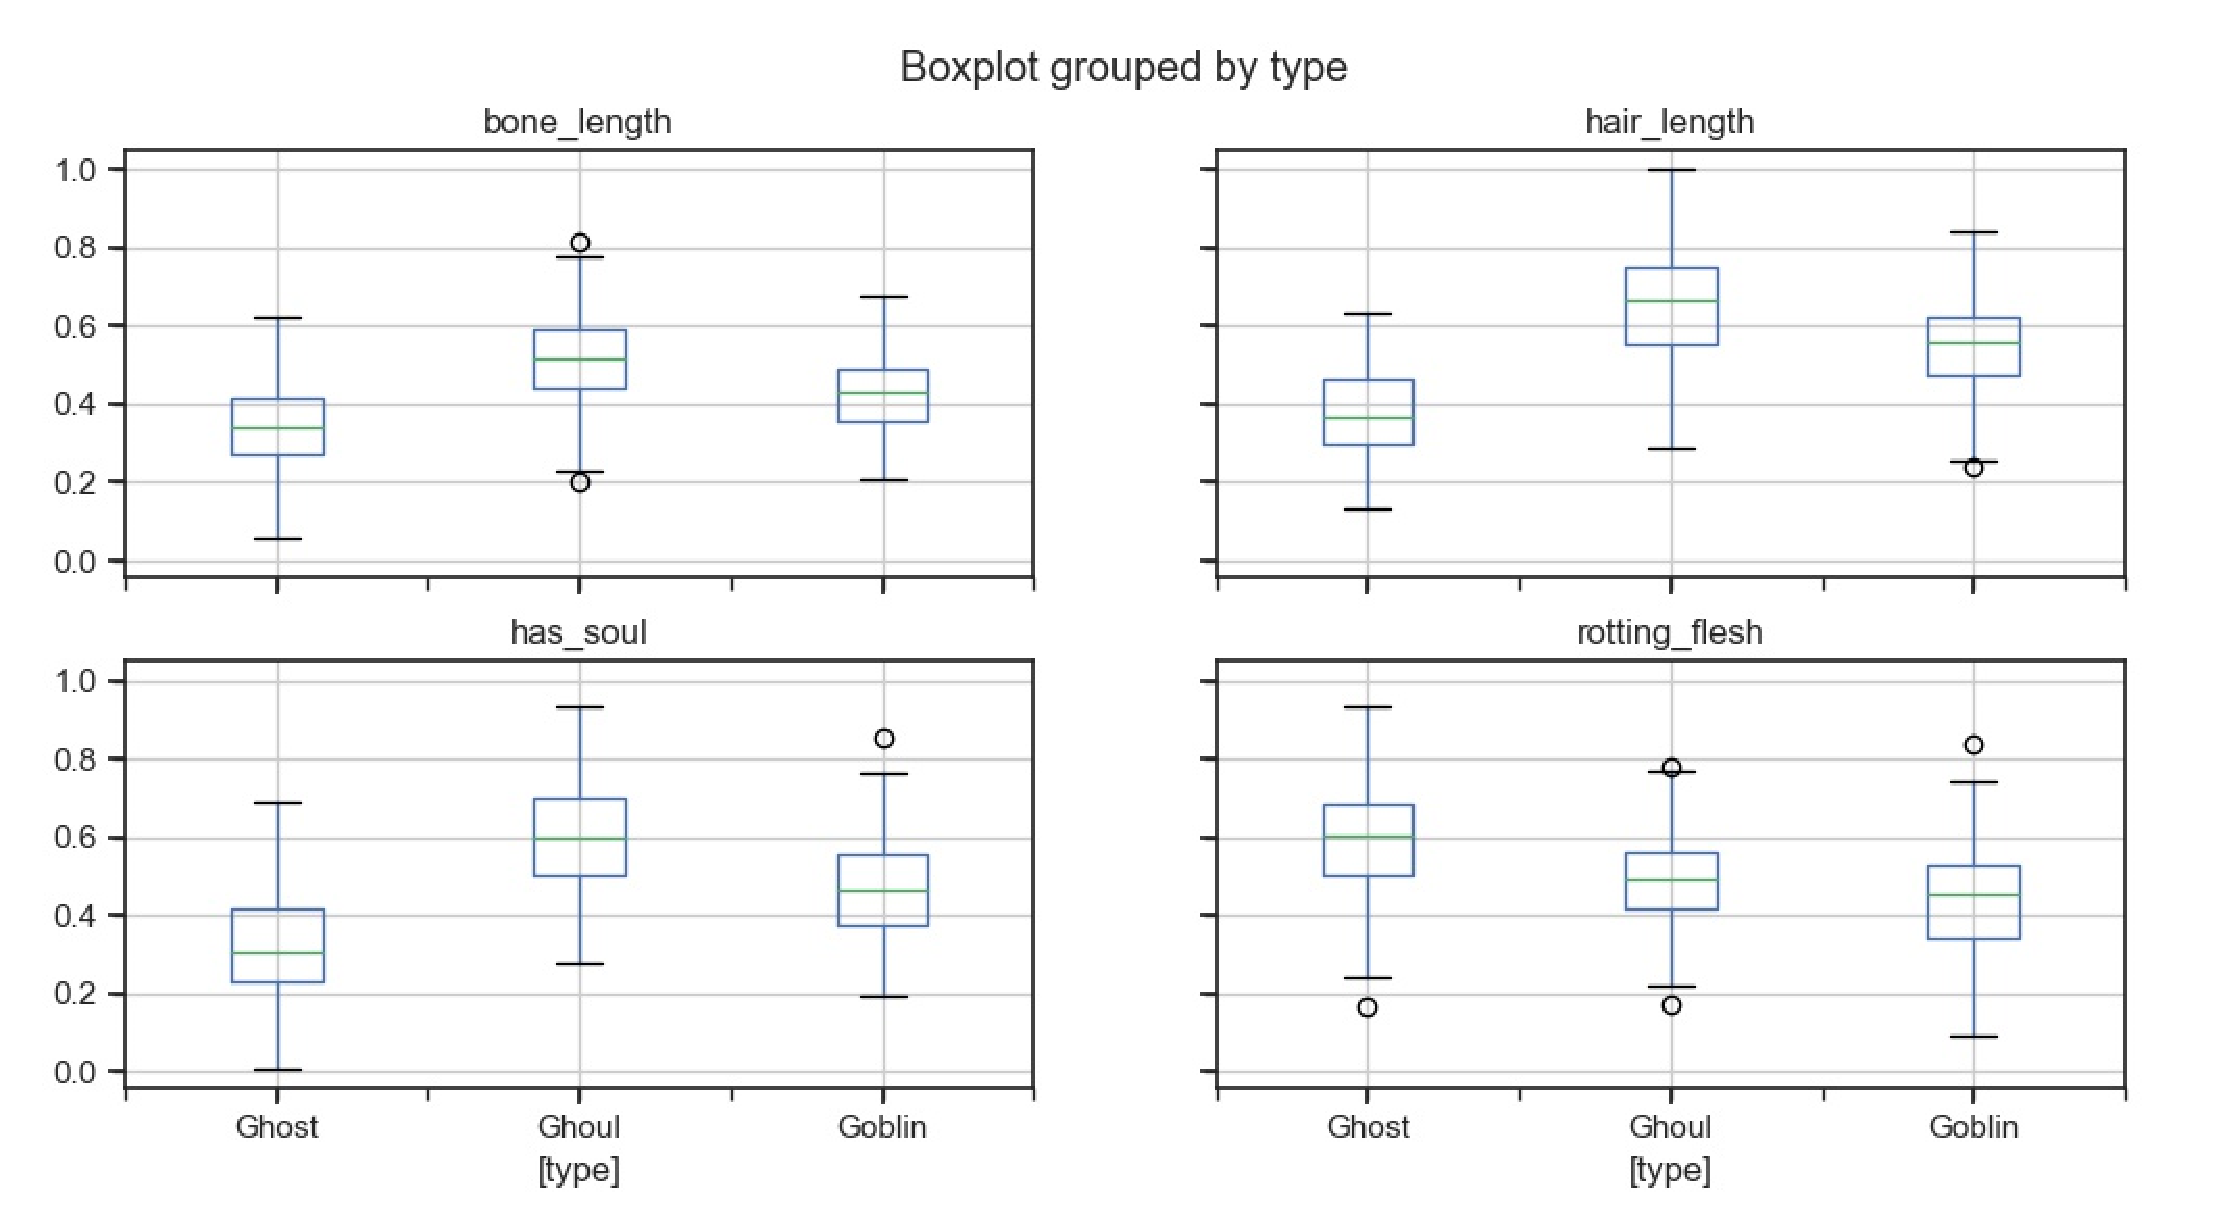
\includegraphics[width=.3\linewidth,height=.25\linewidth]{figures/boxplot.eps}	
	\end{center}
	\vspace{.3cm}
}
%%%%%%%%%% -------------------------------------------------------------------- %%%%%%%%%%


%%%%%%%%%% -------------------------------------------------------------------- %%%%%%%%%%

%\note{Note with default behavior}

%\note[targetoffsetx=12cm, targetoffsety=-1cm, angle=20, rotate=25]
%{Note \\ offset and rotated}

 % First column - second block


%%%%%%%%%% -------------------------------------------------------------------- %%%%%%%%%%
\block{Feature Engineering}{
  	Some of attributes show clusters: 
  	hair\_length and has\_soul, 
  	hair\_length and bone\_length. 
  	So create new variables 
  	with multiplication of these columns: 
  \vspace{.5cm}	
  	\begin{description}
  		\item[hair\_soul] ’hair\_length’ * ’has\_soul’
  		\item[hair\_bone] 'hair\_length' * 'bone\_length]'
  		\item[bone\_soul] 'row[bone\_length' * 'has\_soul'
  		\item[hair\_soul\_bone]  'hair\_length' * 'has\_soul' * 'bone\_length' 
  	\end{description}
  \vspace{.5cm}
    Using the Feature Importance 
    this function of Random Forest
    to select the most important features
    to form a new train data.
    The two picture, one is pairplot 
    which is ploted by using new features data.
    another is the bar plot which shows 
    the importance of features
  	\vspace{.5cm}
  	\begin{center}
  		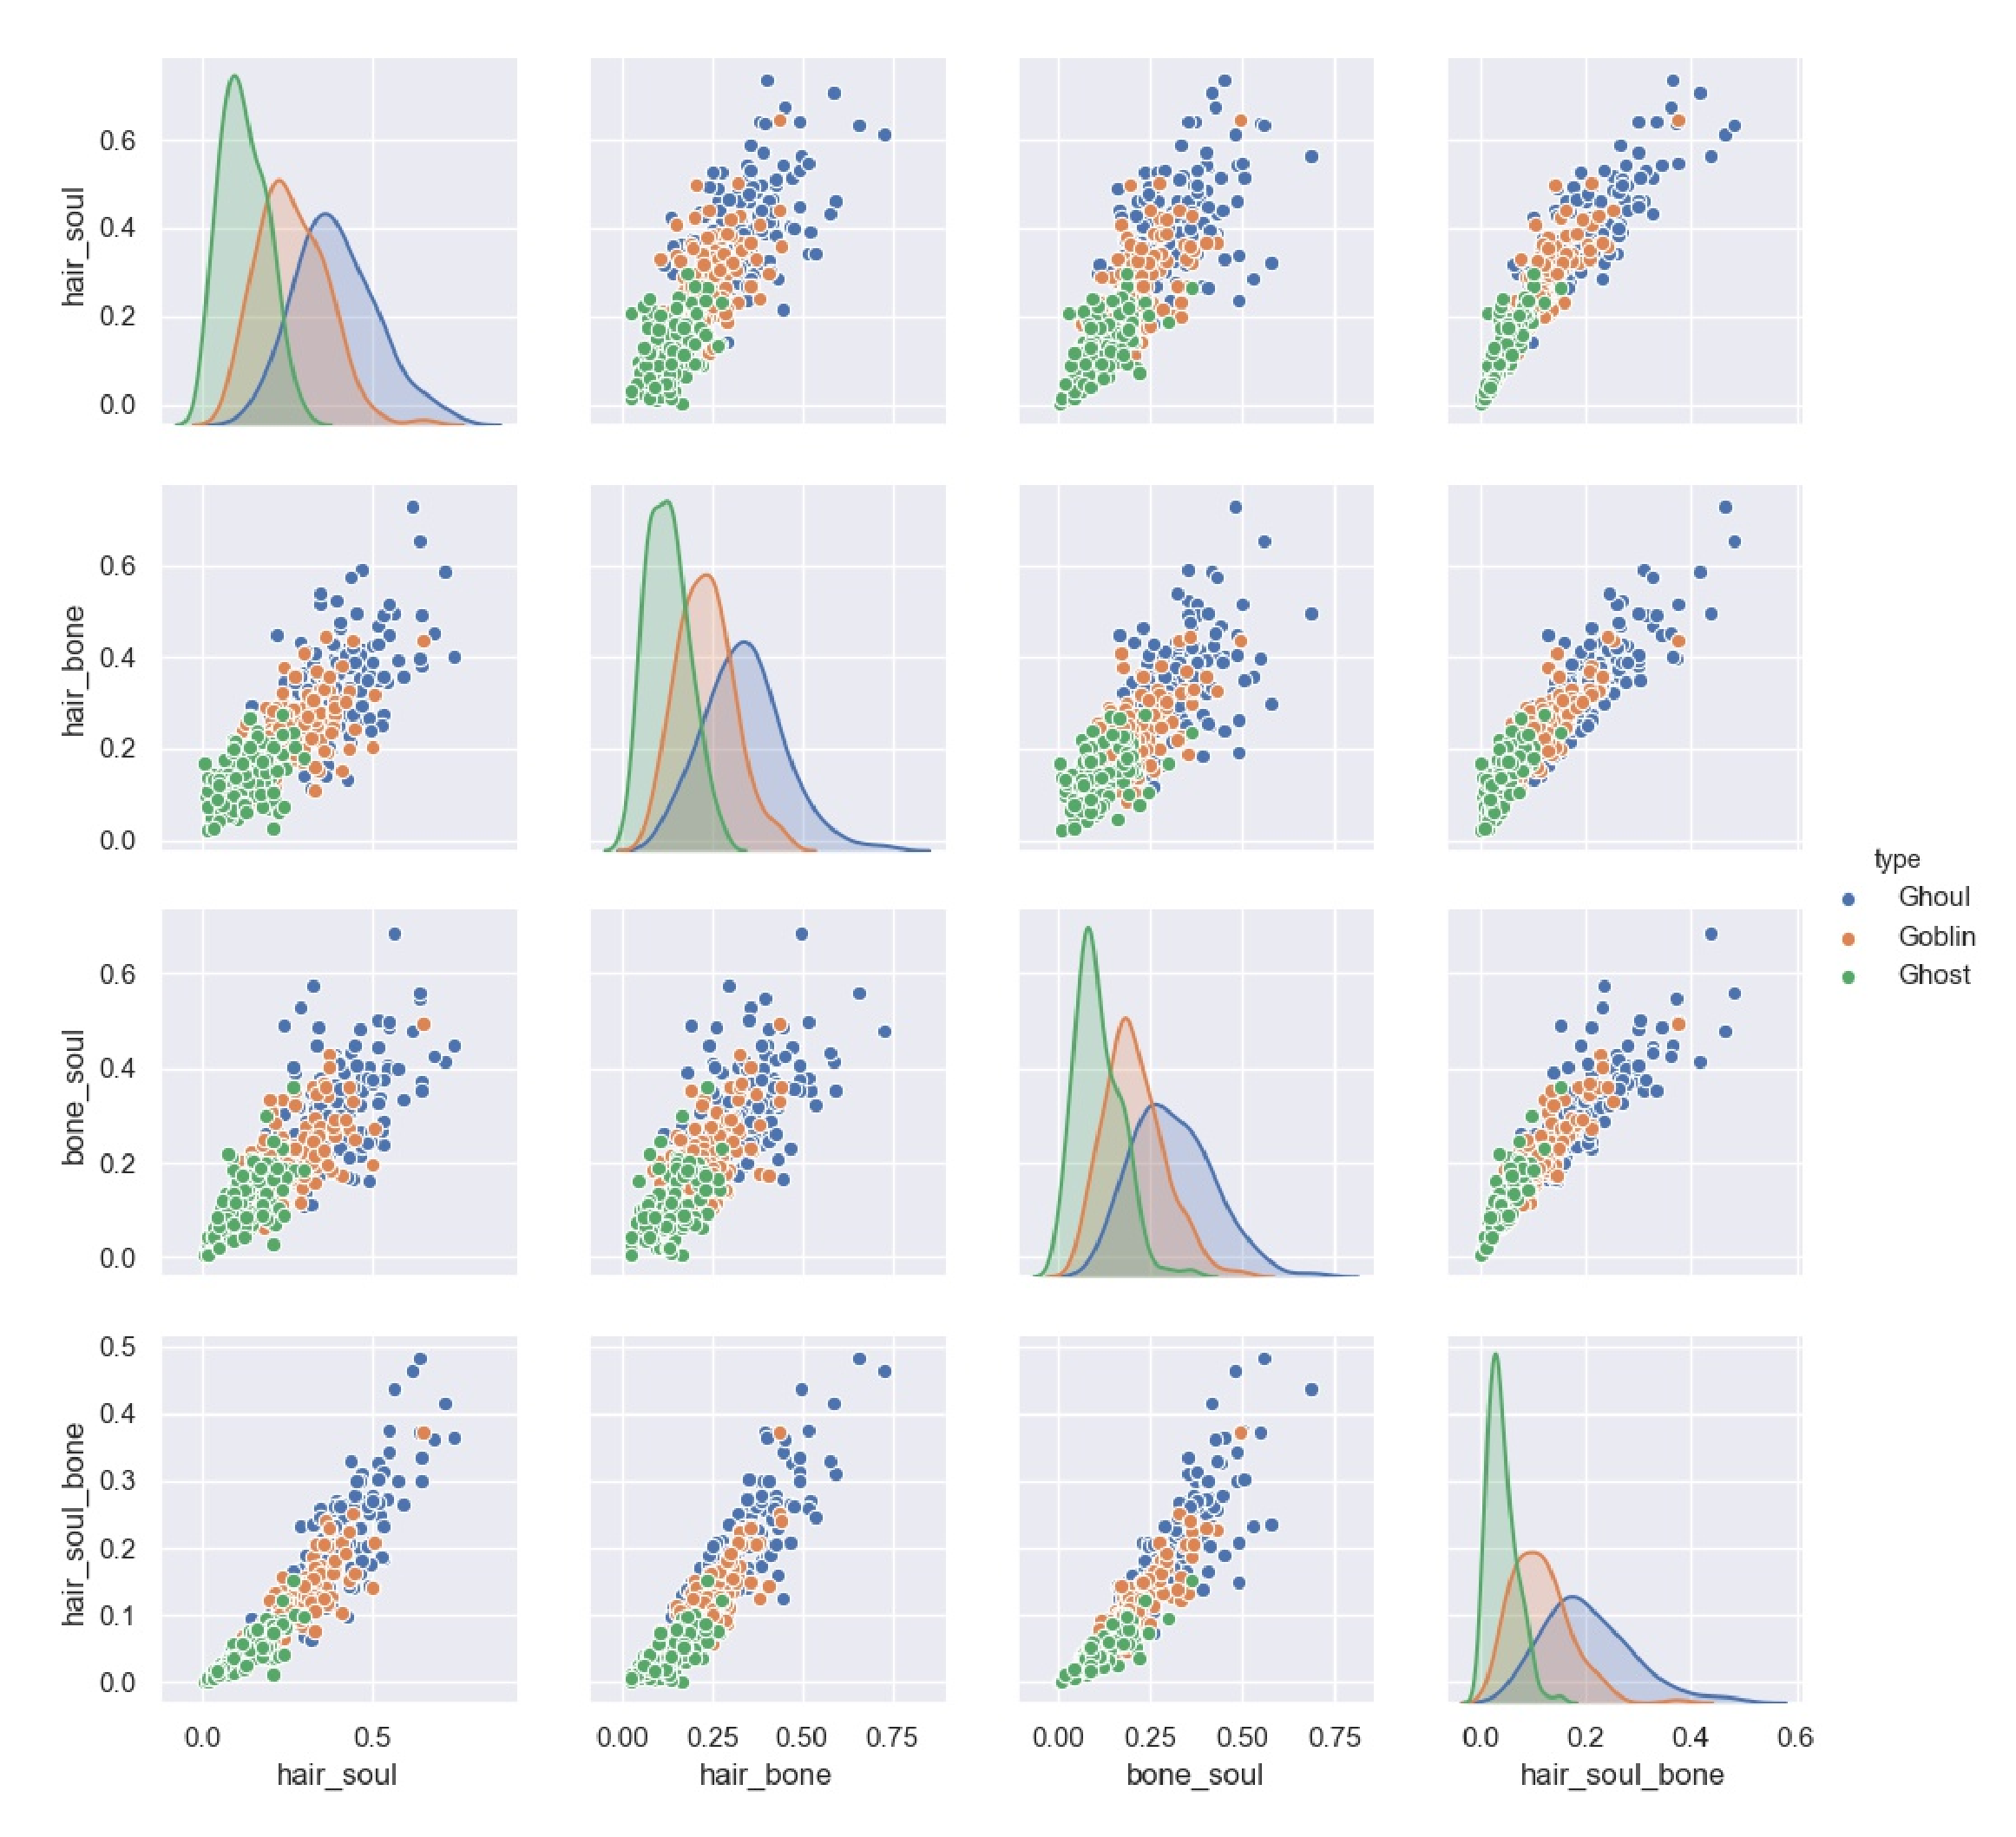
\includegraphics[width=.3\linewidth]{figures/hist_1.eps}
  		\quad
  		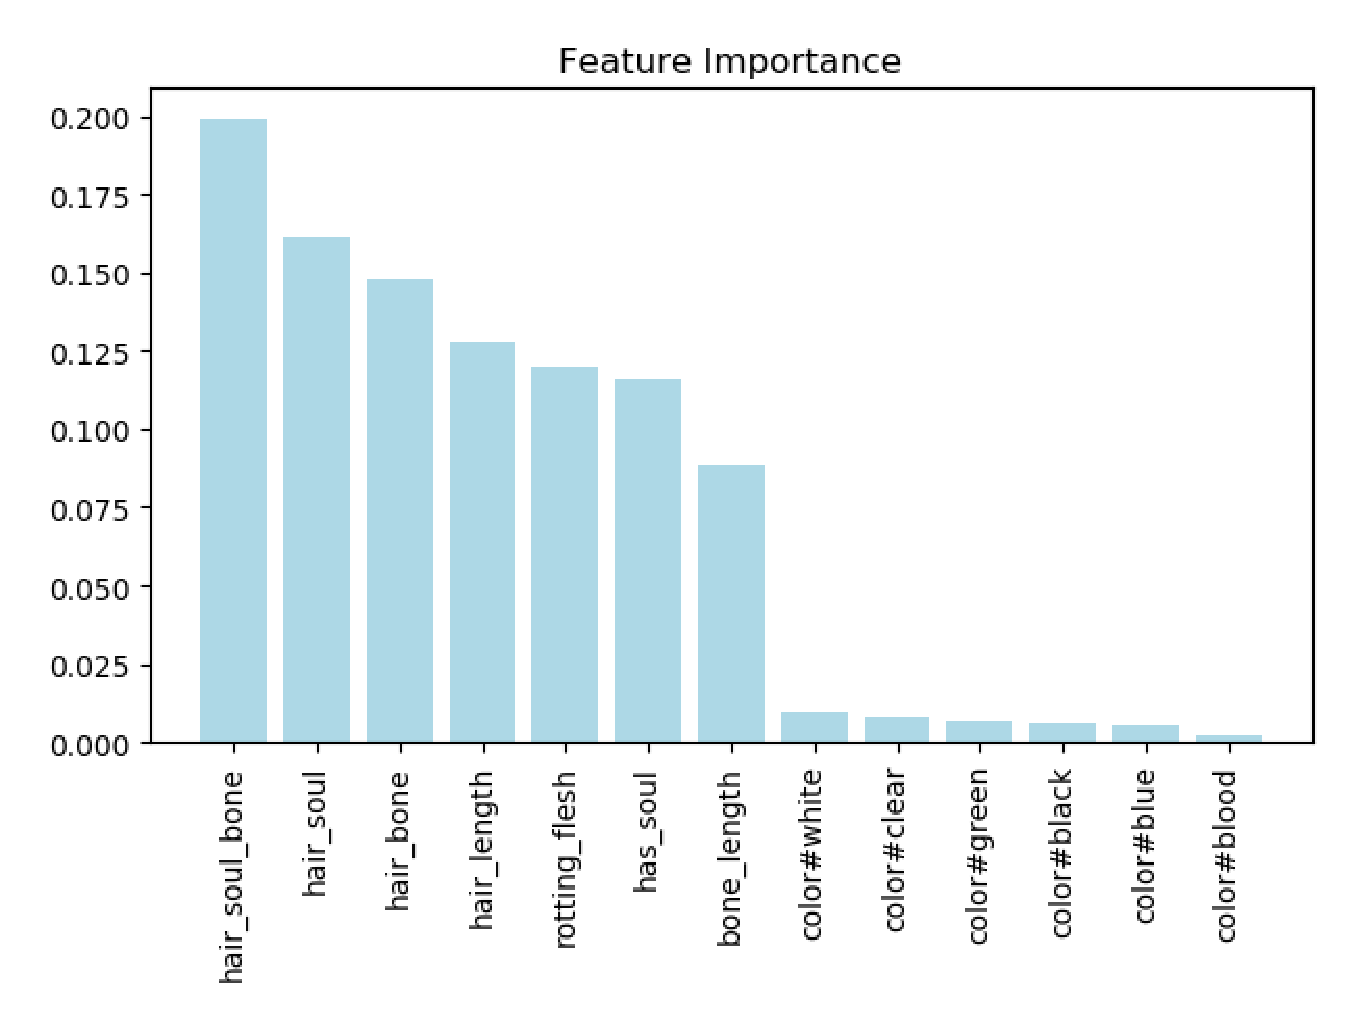
\includegraphics[width=.3\linewidth]{figures/FEATURE.eps}
  	\end{center}
}
%%%%%%%%%% -------------------------------------------------------------------- %%%%%%%%%%


% SECOND column
\column{0.5}
 %Second column with first block's top edge aligned with with previous column's top.

%%%%%%%%%% -------------------------------------------------------------------- %%%%%%%%%%
\block{Algorithm}{
	Choose the following algorithms, 
	use original train data and 
	new train data to train the models,
	and determine a set of optimal parameters 
	through Grid Search.
	Because the train data is relatively small, 
	a ten-fold cross-validation is used.
	\vspace{.5cm}
	\begin{itemize}
		\item RandomForest 
		\item LogisticRegression
		\item SVC
		\item KNeighbors 
		\item XGBoost
		\item Netual Network
	\end{itemize}
	\vspace{.5cm}
	Take the trained models as
	the base models of ensemble model,
	and average the prediction results 
	by using voting
	\vspace{.5cm}
}
%%%%%%%%%% -------------------------------------------------------------------- %%%%%%%%%%
% Second column - first block
\block{Algorithm}{
	\begin{algorithm}[htbp]
		\small
		\caption{Features Selection}
		\label{alg:features_selection}
		\begin{algorithmic}[1]
			
		\end{algorithmic}
		%\caption{Feature Selection Algorithm}
	\end{algorithm}
	
}

%%%%%%%%%% -------------------------------------------------------------------- %%%%%%%%%%
\block[titleleft]{Experiment Result}
{
	The tables below are the metrics classification report 
	of ensemble model in original and new train data.
	\vspace{.4cm}
	\begin{itemize}
  		\item Metrics Classification Report of Ensemble Model in original train data
	\end{itemize}
	\vspace{.5cm}
	\begin{center}
		\begin{tabular}{ccccc}
			\hline
			& precision  &  recall & f1-score &  support\\
			\hline
			Ghost   &    0.80   &   0.83  & 0.82 & 24\\
			Ghoul  &  0.88  &  0.79  &   0.84   &   29\\
			Goblin  &   0.67  &  0.73 &  0.70  &   22\\
			\hline
			micro avg  &  0.79  &  0.79  & 0.79    &  75\\
			macro avg  &  0.78  & 0.78  &  0.78  &  75\\
			weighted avg  &   0.79  &  0.79 &  0.79  &  75\\
			\hline 
			%\bottomrule
		\end{tabular}
	\end{center}
	\vspace{.5cm}

	\begin{itemize}
		\item Metrics Classification Report of Ensemble Model in new train data
	\end{itemize}
	\vspace{.5cm}
	\begin{center}
		\begin{tabular}{ccccc}
			\hline
			&precision & recall & f1-score & support\\
			\hline
			Ghost  &  0.84  &  0.88  & 0.86 &  24\\
			Ghoul  &  0.93  & 0.97 &  0.95 &   29\\
			Goblin  &  0.80 &  0.73  & 0.76  &  22\\
			\hline
			micro avg & 0.87  & 0.87  & 0.87  & 75\\
			macro avg &  0.86  &  0.86 & 0.86 &   75\\
			weighted avg  &  0.86 & 0.87  &  0.86  &  75\\
			\hline 
			%\bottomrule
		\end{tabular}
	\end{center}
	\vspace{.5cm}
	It can be observed that ensemble model
	performaces better in new features.
	
}
%%%%%%%%%% -------------------------------------------------------------------- %%%%%%%%%%


% Second column - second block
%%%%%%%%%% -------------------------------------------------------------------- %%%%%%%%%%
\block[titlewidthscale=1, bodywidthscale=1]
{Conclusion}
{
	\begin{description}
		\item[Exploratory Data Analysis] It is an 
		exploratory analysis of the data can 
		 
		provide the necessary conclusions 
		for data processing and modeling.
		\vspace{.5cm}
		\item[Data Preprocessing] This step contains
		dealing with missing data and outliers,
		changing categorical variable 
		into one-hot code and so on.
		\vspace{.5cm}
		\item[Feature Engineering] It's the 
		most important thing.
		Create as more as poosible features,
		then select the most useful features.
		\vspace{.5cm}
		\item[Model Training] The models have 
		many parameters,
		and can use Grid Search to find 
		the optimal paratemers.	
	\end{description}
}
%%%%%%%%%% -------------------------------------------------------------------- %%%%%%%%%%


% Bottomblock
%%%%%%%%%% -------------------------------------------------------------------- %%%%%%%%%%
\colorlet{notebgcolor}{blue!20}
\colorlet{notefrcolor}{blue!20}
\note[targetoffsetx=8cm, targetoffsety=-4cm, angle=30, rotate=15,
radius=2cm, width=.26\textwidth]{
Acknowledgement
\begin{itemize}
    \item
    Thanks!
 \end{itemize}
}

%\note[targetoffsetx=8cm, targetoffsety=-10cm,rotate=0,angle=180,radius=8cm,width=.46\textwidth,innersep=.1cm]{
%Acknowledgement
%}

%\block[titlewidthscale=0.9, bodywidthscale=0.9]
%{Acknowledgement}{
%}
%%%%%%%%%% -------------------------------------------------------------------- %%%%%%%%%%

\end{columns}


%%%%%%%%%% -------------------------------------------------------------------- %%%%%%%%%%
%[titleleft, titleoffsetx=2em, titleoffsety=1em, bodyoffsetx=2em,%
%roundedcorners=10, linewidth=0mm, titlewidthscale=0.7,%
%bodywidthscale=0.9, titlecenter]

%\colorlet{noteframecolor}{blue!20}
\colorlet{notebgcolor}{blue!20}
\colorlet{notefrcolor}{blue!20}
\note[targetoffsetx=-13cm, targetoffsety=-12cm,rotate=0,angle=180,radius=8cm,width=.96\textwidth,innersep=.4cm]
{
\begin{minipage}{0.3\linewidth}
\centering

\includegraphics[width=24cm]{logos/tulip-wordmark.eps}
\end{minipage}
\begin{minipage}{0.7\linewidth}
{ \centering
 Flip 00 project final report,
  27/10/2019, Nanjing, China
}
\end{minipage}
}
%%%%%%%%%% -------------------------------------------------------------------- %%%%%%%%%%


\end{document}

%\endinput
%%
%% End of file `tikzposter-template.tex'.
